\documentclass[11pt,a4paper]{article}

\usepackage[a4paper,margin=1in]{geometry}
\usepackage[T1]{fontenc}
\usepackage[utf8]{inputenc}
\usepackage{lmodern}
\usepackage{setspace}
\usepackage{graphicx}
\usepackage{subcaption}
\usepackage{booktabs}
\usepackage{array}
\usepackage{longtable}
\usepackage{pdflscape}
\usepackage{adjustbox}

\graphicspath{{results/plots/}}
\setstretch{1.08}
\setlength{\parskip}{0.45em}
\setlength{\parindent}{0pt}
\setlength{\textfloatsep}{10pt plus 2pt minus 2pt}
\setlength{\floatsep}{8pt plus 2pt minus 2pt}

\begin{document}

\begin{titlepage}
\thispagestyle{empty}
\begin{center}

\vspace*{1.1cm}

{\fontsize{24}{30}\selectfont\bfseries
Experimentation and Expansion of\\
Enhanced Credit Risk Prediction Using\\
Deep Learning and SMOTE-ENN\\
Resampling\par}

\vspace{0.7cm}

{\fontsize{15}{20}\selectfont\bfseries
A Cross-Dataset Analysis of Performance,\\
Generalization, Imbalance Handling, and Explainability\par}

\vspace{2.2cm}

\noindent
\begin{minipage}[t]{0.44\textwidth}
\centering
{\Large\bfseries Abubakar Imran\par}
\vspace{0.15cm}
{\large\itshape Roll No: 23i-2589\par}
\vspace{0.15cm}
{\large\itshape i232589@isb.nu.edu.pk\par}
\end{minipage}
\hfill
\begin{minipage}[t]{0.44\textwidth}
\centering
{\Large\bfseries Waqas Ahmed\par}
\vspace{0.15cm}
{\large\itshape Roll No: 23i-2540\par}
\vspace{0.15cm}
{\large\itshape i232540@isb.nu.edu.pk\par}
\end{minipage}

\vspace{0.7cm}

{\Large\bfseries Muhammad Huzaifa Khalid\par}
\vspace{0.15cm}
{\large\itshape Roll No: 23i-2508\par}
\vspace{0.15cm}
{\large\itshape i232508@isb.nu.edu.pk\par}

\vfill

{\Large Department of Artificial Intelligence \& Data Science\par}
\vspace{0.15cm}
{\Large School of Computing, FAST-NUCES\par}
\vspace{0.15cm}
{\Large\itshape CS-4112 Deep Learning\par}
\vspace{0.15cm}
{\Large April 2026\par}

\end{center}
\end{titlepage}

\section{Introduction}
Credit risk prediction is an imbalanced binary classification problem with direct operational consequences: false negatives can expose lenders to default risk, while false positives can reject creditworthy applicants. In Assignment 2, the core paper reproduction focused on testing whether SMOTE-ENN consistently improved deep-learning performance on the Australian and German credit datasets. The reproduced evidence did not confirm the paper's headline claim, which motivated a broader follow-up study rather than a narrow rerun.

This report presents that expansion. The experiment adds the UCI Default of Credit Card Clients dataset and compares four imbalance-handling conditions across three neural architectures: baseline binary cross-entropy (BCE), SMOTE-ENN with BCE, class-weighted BCE, and focal loss. The central research question, taken directly from the experiment configuration, is: \emph{Does SMOTE-ENN consistently improve deep learning credit-risk prediction across datasets, or do loss-based imbalance-handling methods generalize better by preserving the original data distribution?}

The working hypothesis was that loss-based imbalance handling, especially weighted BCE and focal loss, would generalize more stably than SMOTE-ENN because these methods preserve the original training distribution instead of altering it through synthetic oversampling and edited-nearest-neighbor cleaning. The report answers that question using only the saved Assignment 3 artifacts in \texttt{Assignment-3/results}; all tables, figures, and metric values reported below come from those exported files.

\section{Background and Paper Summary}
The target paper, \emph{Enhanced credit risk prediction using deep learning and SMOTE-ENN resampling}, evaluates deep neural architectures for credit-risk prediction under both original and resampled training data. According to the paper summary already documented in the Assignment 2 report, the original study compares MLP, CNN, LSTM, GRU, and GNN variants on the Australian and German datasets, uses 10-fold cross-validation, and reports accuracy, sensitivity, and specificity as the primary metrics. Its central empirical claim is that GRU combined with SMOTE-ENN is the best-performing configuration, with reported accuracy values of 0.926 on the Australian dataset and 0.899 on the German dataset after resampling.

Conceptually, the paper's pipeline is straightforward:
\begin{center}
Preprocessing $\rightarrow$ SMOTE-ENN $\rightarrow$ Deep Model Training $\rightarrow$ Evaluation $\rightarrow$ SHAP
\end{center}
The paper also frames SHAP as the explanation method applied to the strongest model. That is important in the context of this course project because the study sits at the boundary between predictive performance and post-hoc explainability.

However, the Assignment 2 reproduction already identified several reproducibility concerns that remain relevant here:
\begin{itemize}
    \item The semantic description of the Australian dataset in the paper does not align cleanly with the anonymized official file.
    \item The German results section contains a substantive contradiction: some narrative passages imply that pre-resampling or simpler resampling variants outperform SMOTE-ENN, while the headline tables favor GRU + SMOTE-ENN.
    \item GNN implementation details are under-specified, especially around graph construction, which makes faithful reproduction difficult.
\end{itemize}

For these reasons, the Assignment 3 expansion keeps the most defensible subset of the original experimental idea: MLP, LSTM, and GRU, with a controlled comparison between data-level and loss-level imbalance handling, and with SHAP used as a post-hoc explanatory layer for the strongest aggregate configurations.

\section{Reproduction Summary}
The Assignment 2 reproduction did \emph{not} support the original paper's strongest conclusion. Instead of showing a robust advantage for SMOTE-ENN, the reproduction found that baseline models achieved higher mean validation accuracy on both reproduced datasets. Table~\ref{tab:reproduction-summary} summarizes the main result that motivated the current expansion.

\begin{table}[htbp]
\centering
\small
\caption{Assignment 2 reproduction summary from the uploaded report.}
\label{tab:reproduction-summary}
\begin{tabular}{lccc}
\toprule
Dataset & Baseline Mean Accuracy & SMOTE-ENN Mean Accuracy & Difference \\
\midrule
Australian & 0.893 & 0.881 & -0.012 \\
German & 0.890 & 0.877 & -0.013 \\
\bottomrule
\end{tabular}
\end{table}

That earlier reproduction also reported that resampled models often reduced training loss while increasing validation loss, suggesting a generalization problem rather than a pure optimization problem. In short, the earlier report raised a stronger question than ``can the paper be rerun?'' It suggested a scientific question: if SMOTE-ENN is not robustly beneficial, which imbalance-handling strategy transfers best across credit datasets with different sizes and class ratios? Assignment 3 was designed to answer that question directly.

\section{Proposed Method}
The proposed method extends the earlier reproduction in three ways.

First, it introduces a third benchmark: the UCI Default of Credit Card Clients dataset. This addition matters because it is much larger than the Australian and German datasets and is also more imbalanced, making it a better stress test for whether an imbalance-handling strategy scales beyond small benchmark settings.

Second, the experiment compares four conditions instead of only two:
\begin{itemize}
    \item \textbf{Baseline}: standard BCE on the original fold data.
    \item \textbf{SMOTE-ENN}: resampling applied to the training fold before fitting.
    \item \textbf{Weighted BCE}: BCE with a positive-class weight computed from the training fold as $\texttt{negatives} / \texttt{positives}$.
    \item \textbf{Focal Loss}: focal loss with $\gamma = 2.0$ and an $\alpha$ term derived from the training-fold positive rate and clipped into the interval $[0.05, 0.95]$.
\end{itemize}

Third, the expanded study evaluates a broader set of metrics. In addition to the paper-aligned measures (accuracy, sensitivity, specificity), it reports F1, ROC-AUC, PR-AUC, balanced accuracy, validation loss, training dynamics, paired statistical tests, confusion matrices, and SHAP-based feature importance summaries. This makes the analysis more appropriate for class-imbalanced credit-risk prediction, where overall accuracy alone can be misleading.

The resulting design tests a sharper hypothesis than the original paper: SMOTE-ENN may improve minority exposure, but loss-based methods may generalize better because they preserve the original feature distribution while still reweighting the learning objective.

\section{Experimental Setup}
\subsection*{Data and Preprocessing}
The three datasets used in Assignment 3 are summarized in Table~\ref{tab:dataset-summary}. The Australian dataset is relatively balanced, the German dataset is moderately imbalanced, and the Default Credit dataset is the most imbalanced of the three. This diversity is important because it reveals whether an imbalance-handling strategy is robust or dataset-specific.

\begin{table}[htbp]
\centering
\scriptsize
\caption{Dataset characteristics exported by the Assignment 3 notebook.}
\label{tab:dataset-summary}
\begin{tabular}{lrrrrrr}
\toprule
Dataset & Rows & Features & Positive Rate & Imbalance Ratio & Categorical & Numerical \\
\midrule
Australian Credit Approval & 690 & 14 & 0.4449 & 1.2476 & 7 & 7 \\
German Credit & 1000 & 24 & 0.3000 & 2.3333 & 0 & 24 \\
UCI Default of Credit Card Clients & 30000 & 23 & 0.2212 & 3.5208 & 3 & 14 \\
\bottomrule
\end{tabular}
\end{table}

Preprocessing was implemented fold-safely. For the Australian dataset, low-cardinality integer-like variables were treated as categorical and one-hot encoded after most-frequent imputation, while numerical features were median-imputed and standardized. The German numeric file was median-imputed and standardized across all columns. For the Default Credit dataset, the loader removed the \texttt{ID} field, consolidated rare \texttt{EDUCATION} and \texttt{MARRIAGE} codes into grouped categories, one-hot encoded nominal features, passed ordinal features through after imputation, and standardized continuous numerical features.

\subsection*{Models, Training, and Environment}
The experiment retained the paper-aligned model families: MLP, LSTM, and GRU. Their hyperparameters were fixed across the study, as shown in Table~\ref{tab:design-summary}. MLP and GRU used Adam, while LSTM used RMSprop. The full run used 10 stratified folds, up to 35 epochs, and early stopping with patience 5 and minimum delta 0.0001.

\begin{table}[htbp]
\centering
\small
\caption{Experimental design summary.}
\label{tab:design-summary}
\begin{tabular}{ll}
\toprule
Component & Details \\
\midrule
Datasets & australian, german, default\_credit \\
Models & mlp, lstm, gru \\
Conditions & baseline, smoteenn, weighted\_bce, focal\_loss \\
Folds & 10 \\
Epochs & 35 \\
Early stopping patience & 5 \\
\bottomrule
\end{tabular}
\end{table}

The saved environment summary shows that the full experiment ran in a Kaggle GPU environment with Python 3.12.12, PyTorch 2.10.0+cu128, scikit-learn 1.6.1, imbalanced-learn 0.14.1, SHAP 0.50.0, and two Tesla T4 GPUs available. Deterministic seeding was enabled where practical, although the notebook explicitly notes that mixed precision and low-level GPU scheduling can still leave minor residual nondeterminism.

\subsection*{Evaluation Protocol}
Every result in this report comes from 10-fold stratified cross-validation. For each fold, the preprocessor was fit on the training split only, the model was trained under one of the four conditions, and evaluation was performed on the untouched validation split. The threshold for binary classification was fixed at 0.5. Primary reporting focused on accuracy, balanced accuracy, F1, and PR-AUC because these together better expose the trade-off between overall correctness and minority-class retrieval.

\section{Results and Analysis}
\subsection*{Overall Best Configurations}
Table~\ref{tab:best-models} shows the strongest aggregate configuration for each dataset according to the exported \texttt{best\_models.csv} summary. The pattern is immediately informative: loss-based methods dominated two of the three datasets, while the most imbalanced and largest dataset favored the baseline GRU by PR-AUC.

\begin{table}[htbp]
\centering
\small
\caption{Best aggregate configuration per dataset from \texttt{best\_models.csv}.}
\label{tab:best-models}
\begin{tabular}{llllrrrr}
\toprule
Dataset & Model & Condition & Accuracy & Bal. Acc. & PR-AUC & ROC-AUC & Val Loss \\
\midrule
australian & mlp & focal\_loss & 0.8623 & 0.8621 & 0.9213 & 0.9351 & 0.0423 \\
default\_credit & gru & baseline & 0.8207 & 0.6543 & 0.5525 & 0.7738 & 0.4316 \\
german & mlp & weighted\_bce & 0.7180 & 0.7195 & 0.6454 & 0.8032 & 0.7485 \\
\bottomrule
\end{tabular}
\end{table}

The central high-level result from \texttt{report\_summary.json} is also unambiguous: loss-based conditions matched or outperformed SMOTE-ENN on PR-AUC in all three datasets, while SMOTE-ENN led in none. Figures~\ref{fig:target-distribution} and~\ref{fig:aggregate-heatmap} help contextualize that finding by showing both the degree of class imbalance and the relative ranking of model-condition pairs.

\begin{figure}[htbp]
\centering
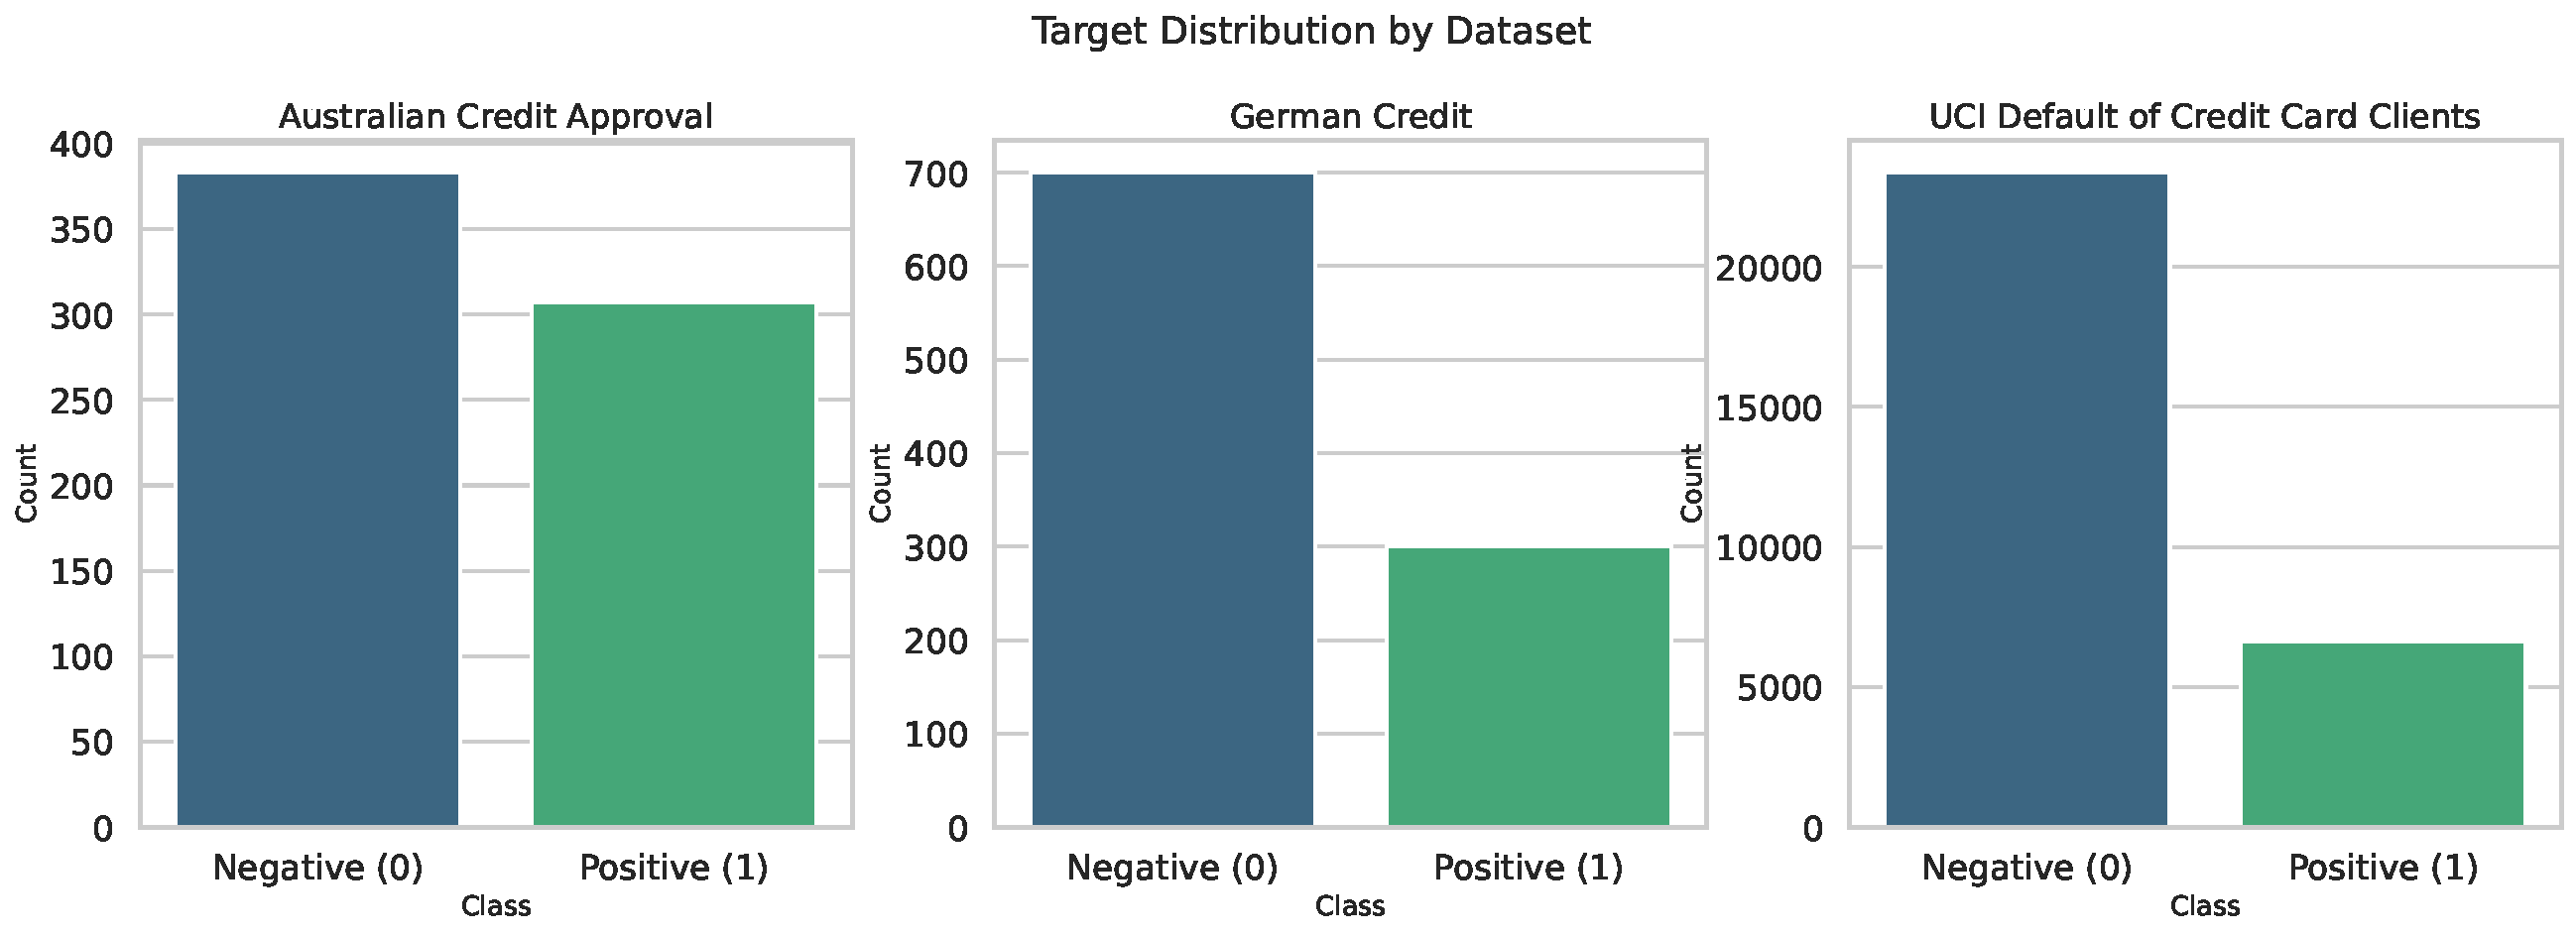
\includegraphics[width=0.78\textwidth]{target_distribution_by_dataset.pdf}
\caption{Class balance differs substantially across datasets, with Default Credit showing the strongest imbalance.}
\label{fig:target-distribution}
\end{figure}

\begin{figure}[htbp]
\centering
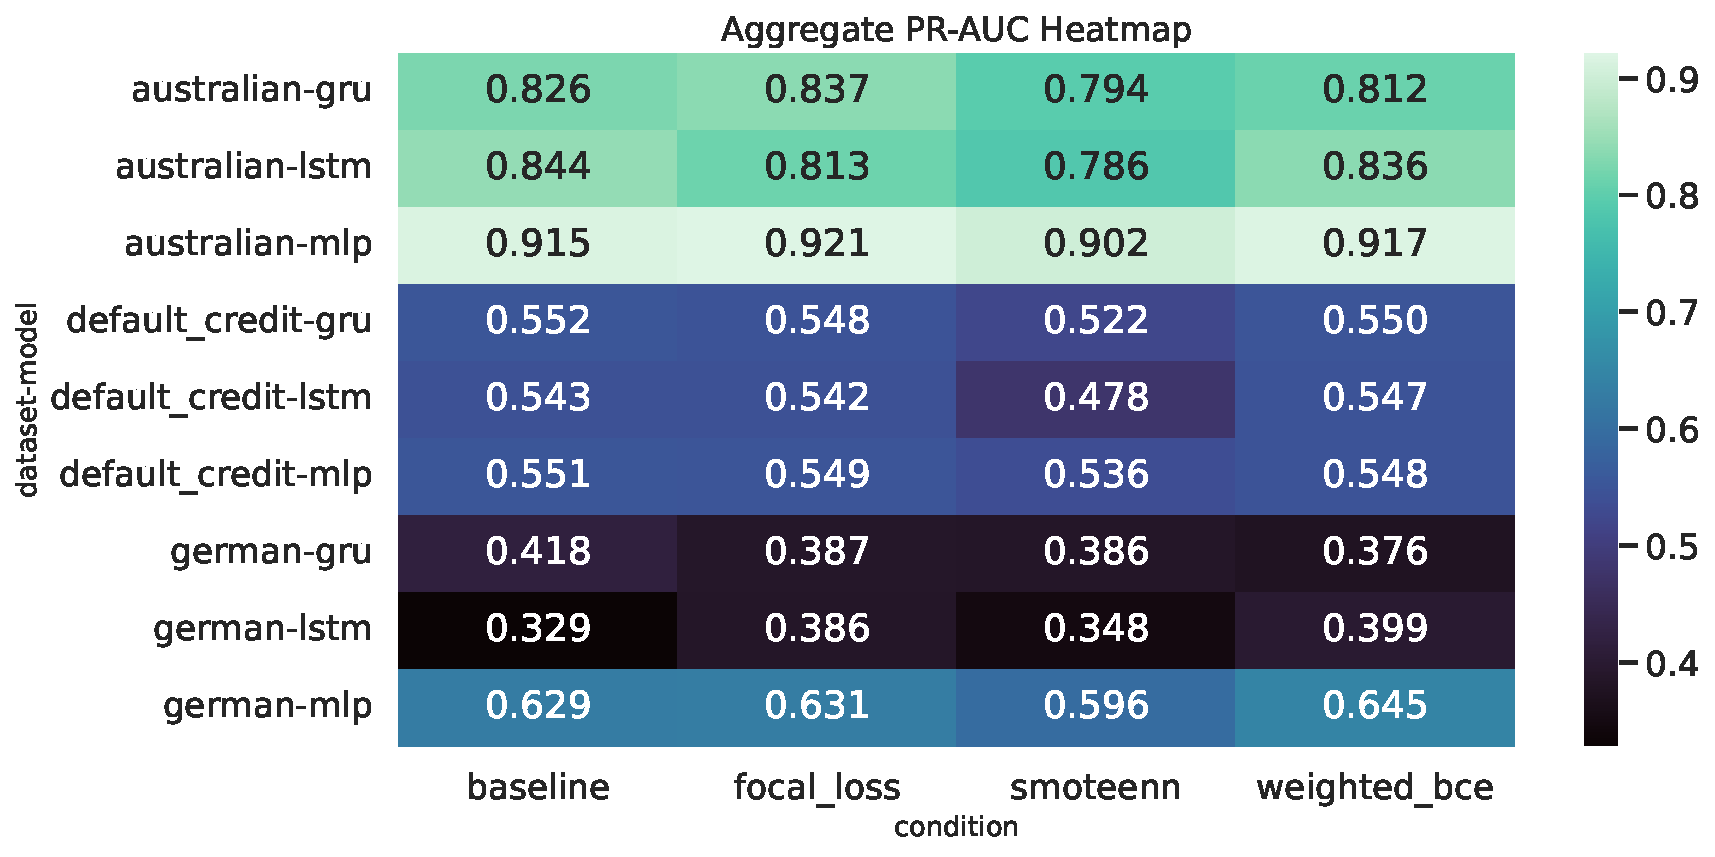
\includegraphics[width=\textwidth]{aggregate_performance_heatmap.pdf}
\caption{Aggregate performance heatmap across all dataset-model-condition combinations.}
\label{fig:aggregate-heatmap}
\end{figure}

\subsection*{Complete Cross-Dataset Metric Tables}
Tables~\ref{tab:australian-all}, \ref{tab:default-all}, and \ref{tab:german-all} report the core aggregate metrics for all 36 model-condition combinations. These values are taken directly from the exported tables and rounded to four decimals for presentation only.

\begin{table}[htbp]
\centering
\scriptsize
\caption{Australian dataset: aggregate metrics for all model-condition pairs.}
\label{tab:australian-all}
\begin{tabular}{llllrrr}
\toprule
Model & Condition & Accuracy & Bal. Acc. & F1 & PR-AUC & ROC-AUC \\
\midrule
GRU & baseline & 0.7899 & 0.7852 & 0.7540 & 0.8261 & 0.8509 \\
GRU & focal\_loss & 0.8014 & 0.7979 & 0.7710 & 0.8371 & 0.8606 \\
GRU & smoteenn & 0.7507 & 0.7417 & 0.6963 & 0.7942 & 0.8236 \\
GRU & weighted\_bce & 0.7652 & 0.7630 & 0.7345 & 0.8123 & 0.8377 \\
LSTM & baseline & 0.8000 & 0.7935 & 0.7614 & 0.8439 & 0.8589 \\
LSTM & focal\_loss & 0.7710 & 0.7681 & 0.7407 & 0.8129 & 0.8401 \\
LSTM & smoteenn & 0.7348 & 0.7201 & 0.6213 & 0.7857 & 0.8198 \\
LSTM & weighted\_bce & 0.7855 & 0.7834 & 0.7591 & 0.8365 & 0.8566 \\
MLP & baseline & 0.8551 & 0.8531 & 0.8314 & 0.9154 & 0.9312 \\
MLP & focal\_loss & 0.8623 & 0.8621 & 0.8442 & 0.9213 & 0.9351 \\
MLP & smoteenn & 0.8435 & 0.8414 & 0.8190 & 0.9022 & 0.9215 \\
MLP & weighted\_bce & 0.8623 & 0.8621 & 0.8426 & 0.9170 & 0.9326 \\
\bottomrule
\end{tabular}
\end{table}

\begin{table}[htbp]
\centering
\scriptsize
\caption{Default Credit dataset: aggregate metrics for all model-condition pairs.}
\label{tab:default-all}
\begin{tabular}{llllrrr}
\toprule
Model & Condition & Accuracy & Bal. Acc. & F1 & PR-AUC & ROC-AUC \\
\midrule
GRU & baseline & 0.8207 & 0.6543 & 0.4674 & 0.5525 & 0.7738 \\
GRU & focal\_loss & 0.7634 & 0.7082 & 0.5328 & 0.5484 & 0.7736 \\
GRU & smoteenn & 0.7243 & 0.6979 & 0.5130 & 0.5218 & 0.7603 \\
GRU & weighted\_bce & 0.7656 & 0.7077 & 0.5325 & 0.5498 & 0.7748 \\
LSTM & baseline & 0.8196 & 0.6532 & 0.4647 & 0.5428 & 0.7694 \\
LSTM & focal\_loss & 0.7669 & 0.7081 & 0.5336 & 0.5421 & 0.7706 \\
LSTM & smoteenn & 0.7266 & 0.6721 & 0.4760 & 0.4778 & 0.7349 \\
LSTM & weighted\_bce & 0.7733 & 0.7062 & 0.5336 & 0.5471 & 0.7708 \\
MLP & baseline & 0.8212 & 0.6530 & 0.4645 & 0.5514 & 0.7798 \\
MLP & focal\_loss & 0.7613 & 0.7103 & 0.5342 & 0.5488 & 0.7795 \\
MLP & smoteenn & 0.6721 & 0.6930 & 0.4966 & 0.5360 & 0.7753 \\
MLP & weighted\_bce & 0.7620 & 0.7096 & 0.5338 & 0.5481 & 0.7804 \\
\bottomrule
\end{tabular}
\end{table}

\begin{table}[htbp]
\centering
\scriptsize
\caption{German dataset: aggregate metrics for all model-condition pairs.}
\label{tab:german-all}
\begin{tabular}{llllrrr}
\toprule
Model & Condition & Accuracy & Bal. Acc. & F1 & PR-AUC & ROC-AUC \\
\midrule
GRU & baseline & 0.7090 & 0.5274 & 0.0921 & 0.4182 & 0.6042 \\
GRU & focal\_loss & 0.5180 & 0.5329 & 0.3929 & 0.3872 & 0.5794 \\
GRU & smoteenn & 0.4270 & 0.5374 & 0.4593 & 0.3859 & 0.5902 \\
GRU & weighted\_bce & 0.5630 & 0.5631 & 0.4235 & 0.3760 & 0.5829 \\
LSTM & baseline & 0.7000 & 0.5000 & 0.0000 & 0.3286 & 0.5341 \\
LSTM & focal\_loss & 0.5190 & 0.5460 & 0.4154 & 0.3861 & 0.5836 \\
LSTM & smoteenn & 0.3180 & 0.5033 & 0.4598 & 0.3478 & 0.5421 \\
LSTM & weighted\_bce & 0.5540 & 0.5805 & 0.4632 & 0.3991 & 0.6137 \\
MLP & baseline & 0.7720 & 0.6943 & 0.5627 & 0.6288 & 0.7988 \\
MLP & focal\_loss & 0.7300 & 0.7386 & 0.6277 & 0.6315 & 0.8044 \\
MLP & smoteenn & 0.6210 & 0.6921 & 0.5821 & 0.5961 & 0.7825 \\
MLP & weighted\_bce & 0.7180 & 0.7195 & 0.6073 & 0.6454 & 0.8032 \\
\bottomrule
\end{tabular}
\end{table}

\subsection*{Per-Dataset Interpretation}
\textbf{Australian.} The Australian dataset produced the strongest overall results in the study, and the best configuration was MLP + focal loss with mean accuracy 0.8623, balanced accuracy 0.8621, ROC-AUC 0.9351, and PR-AUC 0.9213. Weighted BCE was nearly tied on accuracy and balanced accuracy, but focal loss achieved the highest PR-AUC. SMOTE-ENN was not catastrophic on this dataset, but it trailed the strongest loss-based variants across every model family. The paired Wilcoxon tests reinforce that pattern: GRU + focal loss significantly outperformed GRU + SMOTE-ENN on PR-AUC (\(p = 0.0195\)), LSTM baseline significantly outperformed LSTM + SMOTE-ENN on PR-AUC (\(p = 0.0195\)), and MLP + focal loss significantly outperformed MLP + SMOTE-ENN on accuracy, F1, and balanced accuracy (\(p \leq 0.0469\)).

\textbf{Default Credit.} The default-credit results were more nuanced. By PR-AUC, the best configuration was GRU baseline at 0.5525, but weighted BCE and focal loss consistently improved balanced accuracy into the 0.706--0.710 range, compared with roughly 0.653 for baseline MLP and LSTM and 0.654 for baseline GRU. This means the baseline models preserved ranking quality and specificity best, while loss-based methods traded some accuracy for stronger minority-class recall. SMOTE-ENN was clearly the weakest strategy here: for all three model families, PR-AUC under SMOTE-ENN was significantly lower than baseline, focal loss, and weighted BCE. The exported significance table shows Wilcoxon \(p = 0.0020\) for all nine of those PR-AUC comparisons.

\textbf{German.} The German dataset showed the clearest difference between ``best by accuracy'' and ``best by imbalance-aware criteria.'' MLP baseline achieved the highest raw accuracy (0.7720), but its sensitivity was only 0.5000. MLP + weighted BCE delivered the highest PR-AUC (0.6454), while MLP + focal loss achieved the highest balanced accuracy (0.7386). In other words, the loss-based variants improved minority-class behavior while preserving competitive discrimination quality. SMOTE-ENN again underperformed: MLP + weighted BCE significantly exceeded MLP + SMOTE-ENN on PR-AUC (\(p = 0.0371\)) and balanced accuracy (\(p = 0.0273\)), and MLP + focal loss significantly exceeded MLP + SMOTE-ENN on balanced accuracy (\(p = 0.0195\)).

\subsection*{Training Dynamics}
The learning-curve and training-dynamics outputs strongly suggest that SMOTE-ENN often made optimization easier while harming validation performance. Table~\ref{tab:training-contrast} contrasts the best-performing configuration on each dataset with a representative SMOTE-ENN alternative from the same dataset. The Australian and German MLP cases are especially revealing: the resampled models reached very high final training accuracy but substantially lower best validation accuracy, consistent with overfitting to the altered training distribution.

\begin{table}[htbp]
\centering
\small
\caption{Training dynamics contrasts from \texttt{training\_dynamics\_table.csv}.}
\label{tab:training-contrast}
\begin{tabular}{llllrrr}
\toprule
Dataset & Model & Condition & Epochs & Final Train Acc. & Best Val. Acc. & Final Train Loss \\
\midrule
australian & mlp & focal\_loss & 12.0 & 0.8890 & 0.8783 & 0.0365 \\
australian & mlp & smoteenn & 8.6 & 0.9901 & 0.8768 & 0.0324 \\
default\_credit & gru & baseline & 22.9 & 0.8231 & 0.8227 & 0.4261 \\
default\_credit & gru & smoteenn & 11.7 & 0.8118 & 0.7509 & 0.3749 \\
german & mlp & weighted\_bce & 12.1 & 0.7638 & 0.7390 & 0.6544 \\
german & mlp & smoteenn & 7.3 & 0.9306 & 0.6810 & 0.1793 \\
\bottomrule
\end{tabular}
\end{table}

\begin{figure}[htbp]
\centering
\begin{subfigure}[t]{0.32\textwidth}
    \centering
    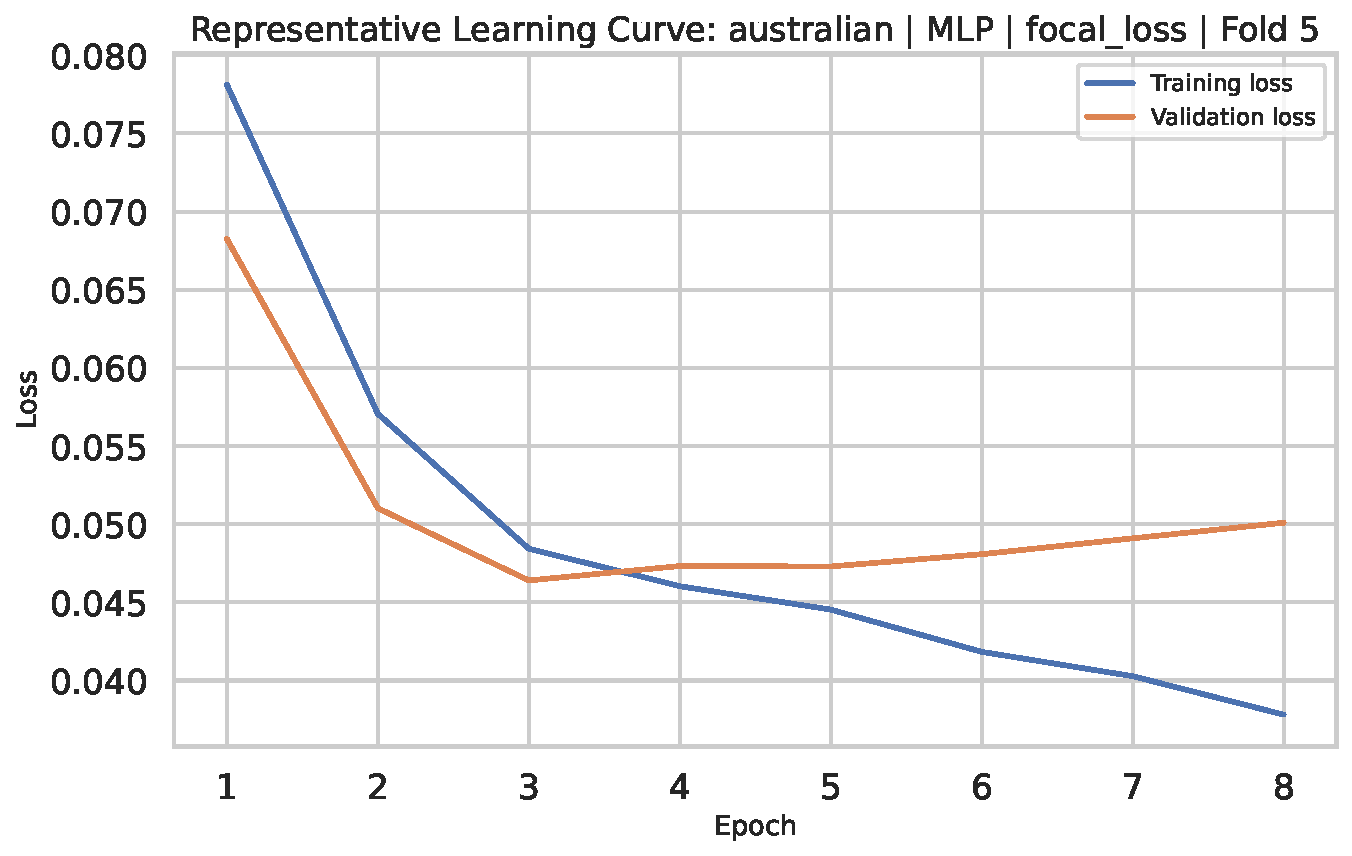
\includegraphics[width=\textwidth]{learning_curve_australian_mlp_focal_loss.pdf}
    \caption{Australian: MLP + focal loss}
\end{subfigure}
\hfill
\begin{subfigure}[t]{0.32\textwidth}
    \centering
    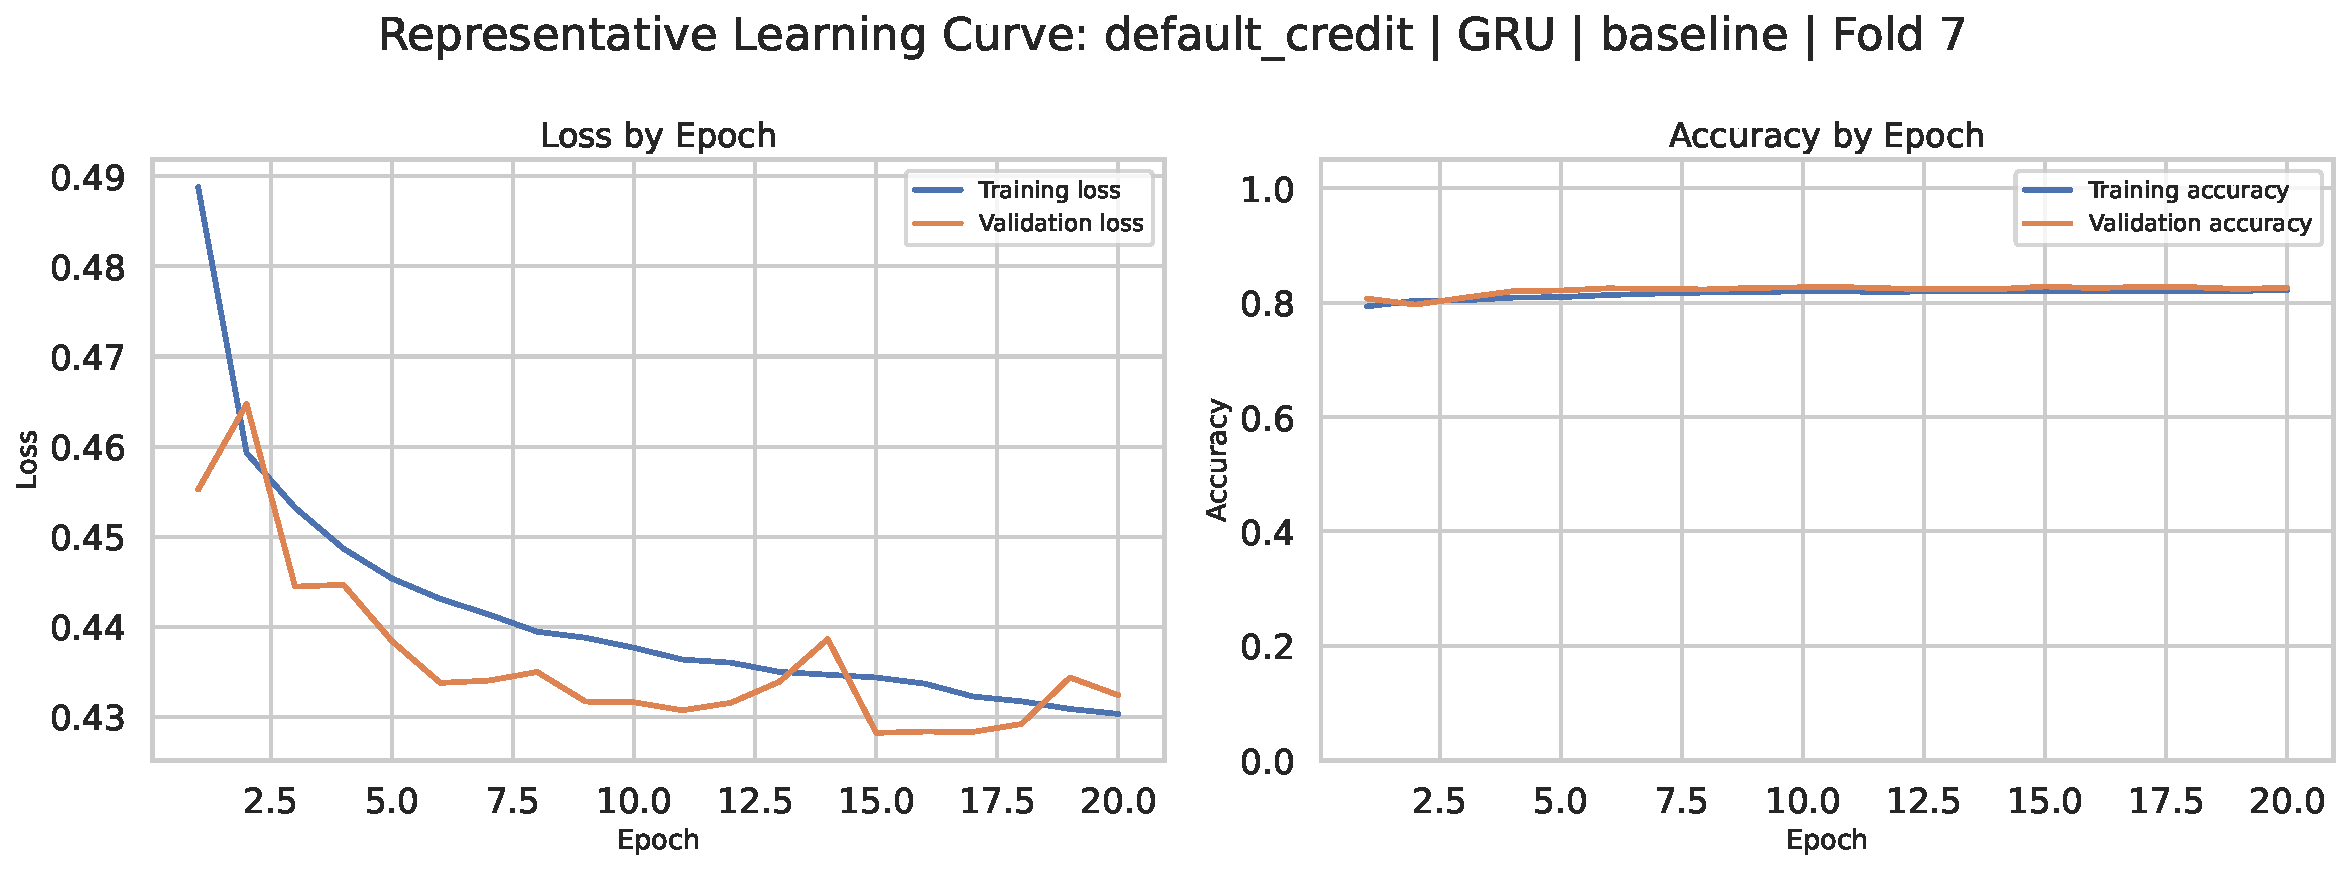
\includegraphics[width=\textwidth]{learning_curve_default_credit_gru_baseline.pdf}
    \caption{Default Credit: GRU baseline}
\end{subfigure}
\hfill
\begin{subfigure}[t]{0.32\textwidth}
    \centering
    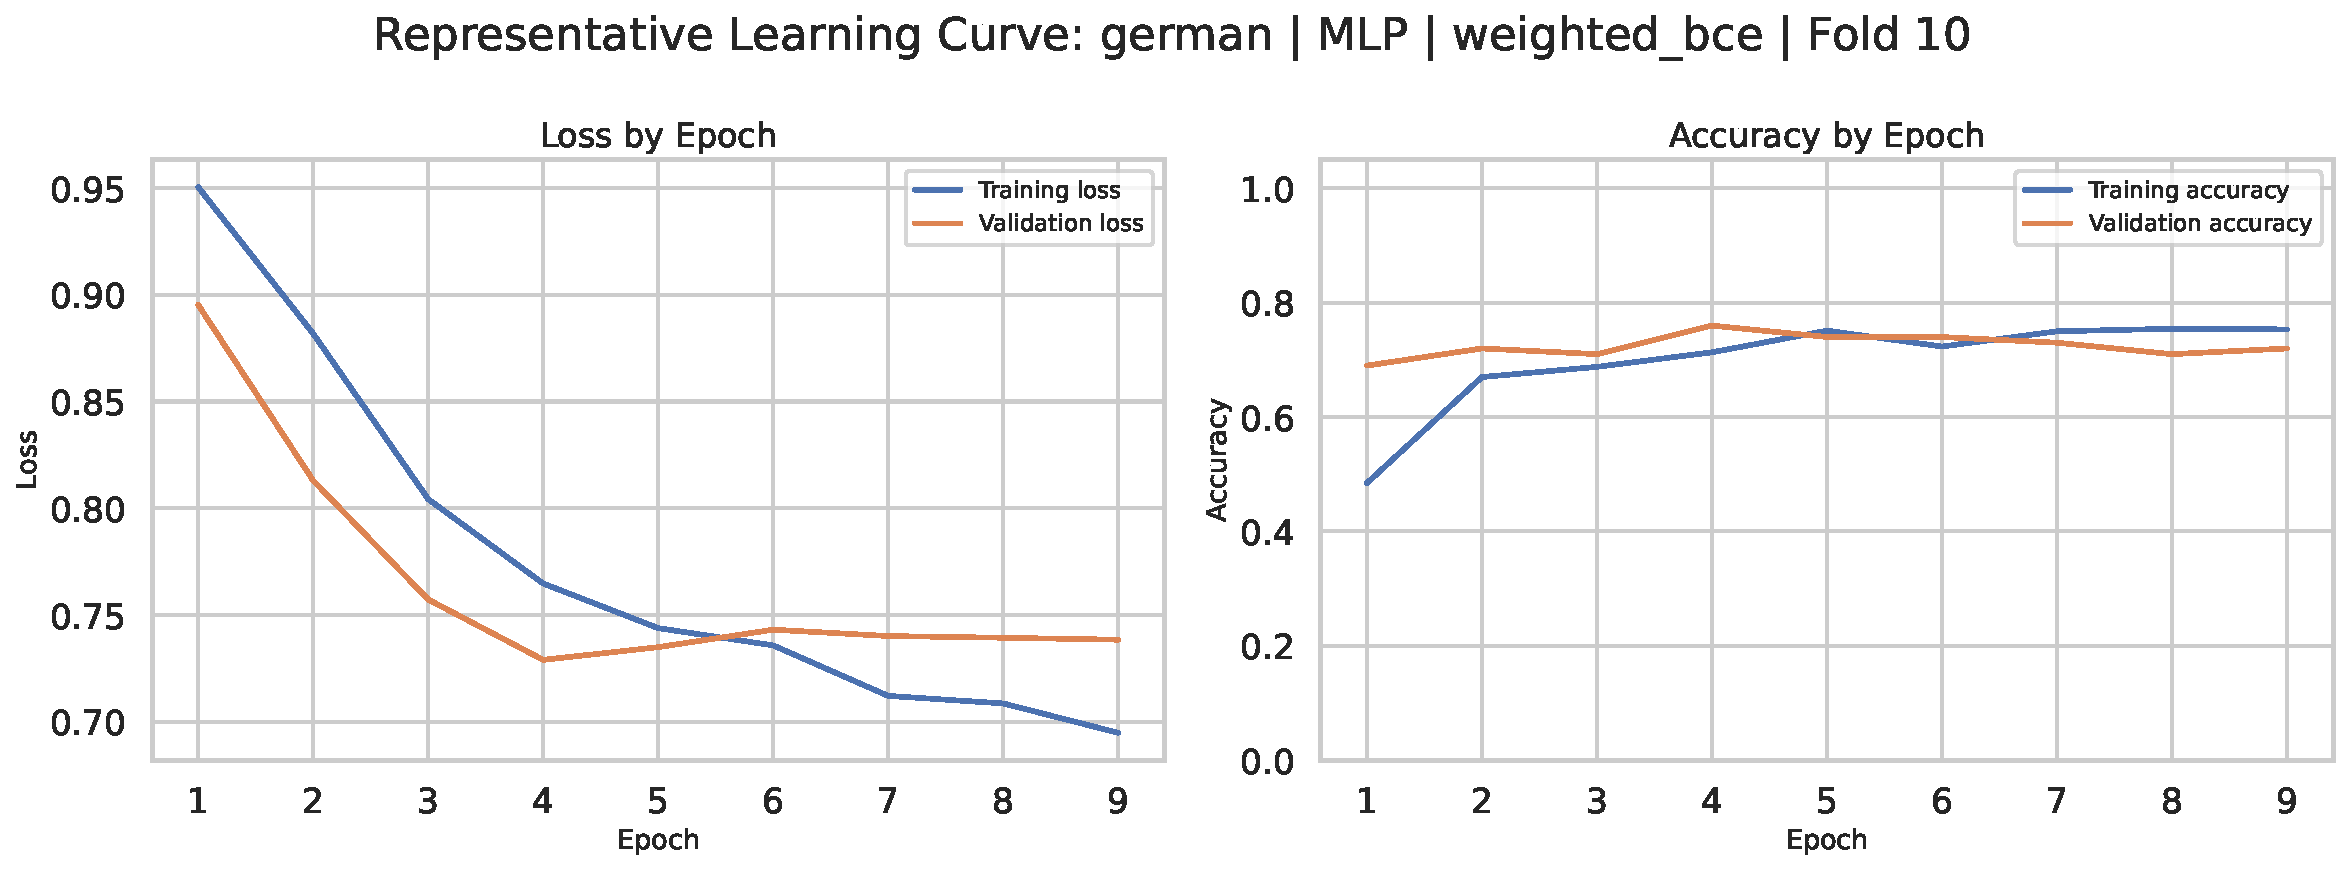
\includegraphics[width=\textwidth]{learning_curve_german_mlp_weighted_bce.pdf}
    \caption{German: MLP + weighted BCE}
\end{subfigure}
\caption{Representative learning curves for the strongest aggregate configuration in each dataset.}
\label{fig:learning-curves}
\end{figure}

\subsection*{Error Profiles and Confusion Patterns}
Error analysis for the best aggregate configuration in each dataset is summarized in Table~\ref{tab:error-analysis}. The Default Credit baseline GRU is the most asymmetric model in the study: its false-positive rate is low (0.0368), but its false-negative rate is high (0.1425), which explains why it leads by PR-AUC and accuracy while trailing loss-based methods on balanced accuracy. German MLP + weighted BCE is the opposite kind of trade-off: it keeps false negatives at 0.0830 but pays for that with a higher false-positive rate of 0.1990.

\begin{table}[htbp]
\centering
\small
\caption{Error analysis for the best aggregate configuration in each dataset.}
\label{tab:error-analysis}
\begin{tabular}{llllrr}
\toprule
Dataset & Model & Condition & Error Type & Count & Rate \\
\midrule
australian & mlp & focal\_loss & correct & 595 & 0.8623 \\
australian & mlp & focal\_loss & false\_negative & 45 & 0.0652 \\
australian & mlp & focal\_loss & false\_positive & 50 & 0.0725 \\
default\_credit & gru & baseline & correct & 24622 & 0.8207 \\
default\_credit & gru & baseline & false\_negative & 4275 & 0.1425 \\
default\_credit & gru & baseline & false\_positive & 1103 & 0.0368 \\
german & mlp & weighted\_bce & correct & 718 & 0.7180 \\
german & mlp & weighted\_bce & false\_negative & 83 & 0.0830 \\
german & mlp & weighted\_bce & false\_positive & 199 & 0.1990 \\
\bottomrule
\end{tabular}
\end{table}

\begin{figure}[htbp]
\centering
\begin{subfigure}[t]{0.32\textwidth}
    \centering
    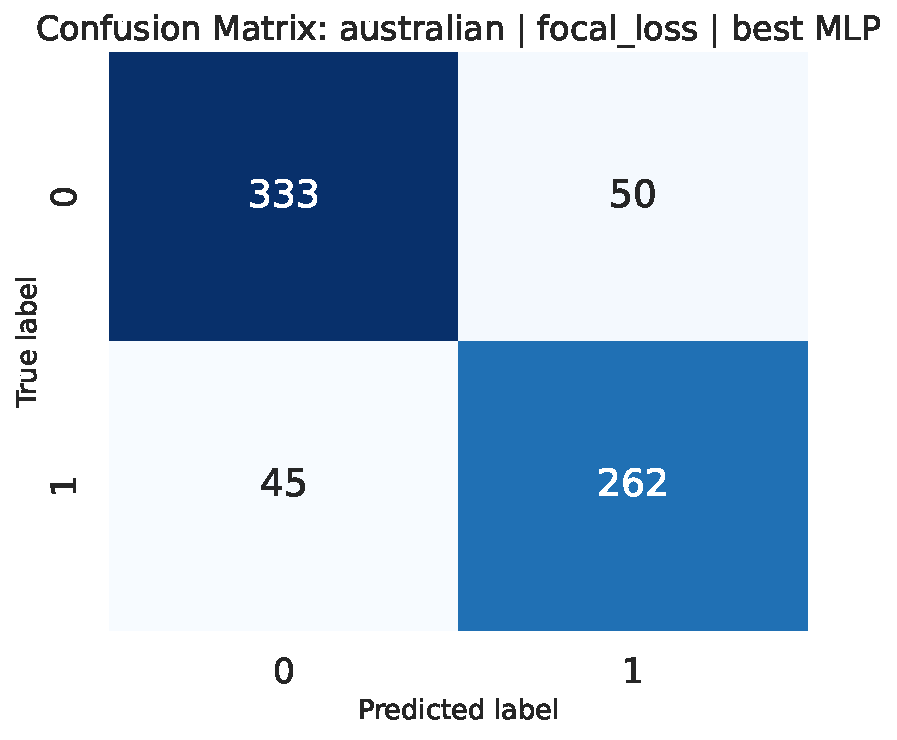
\includegraphics[width=\textwidth]{confusion_matrix_australian_focal_loss.pdf}
    \caption{Australian best model}
\end{subfigure}
\hfill
\begin{subfigure}[t]{0.32\textwidth}
    \centering
    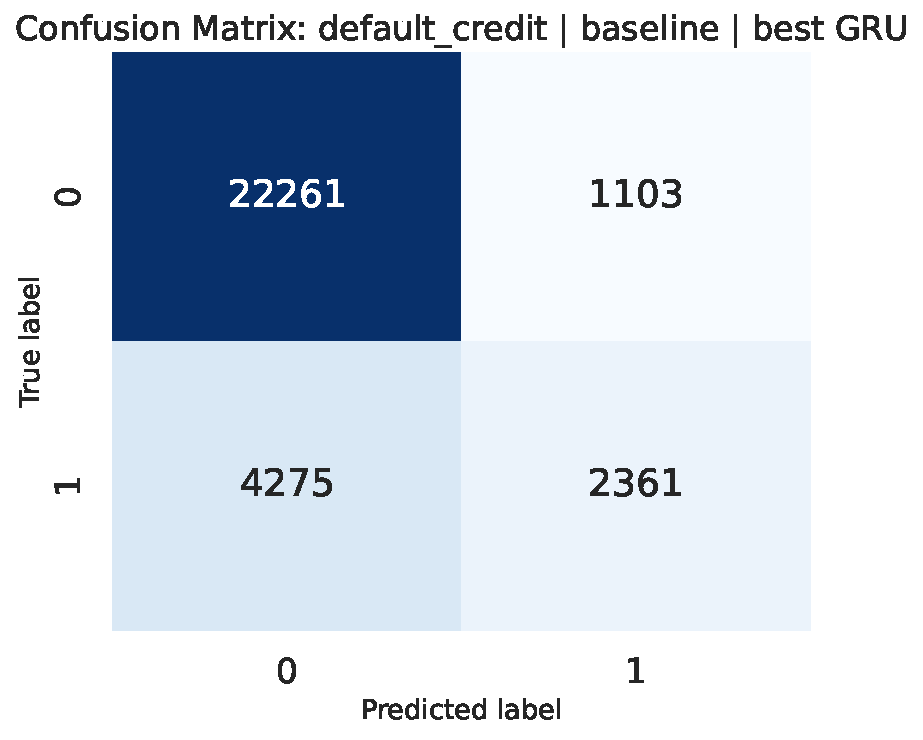
\includegraphics[width=\textwidth]{confusion_matrix_default_credit_baseline.pdf}
    \caption{Default Credit best model}
\end{subfigure}
\hfill
\begin{subfigure}[t]{0.32\textwidth}
    \centering
    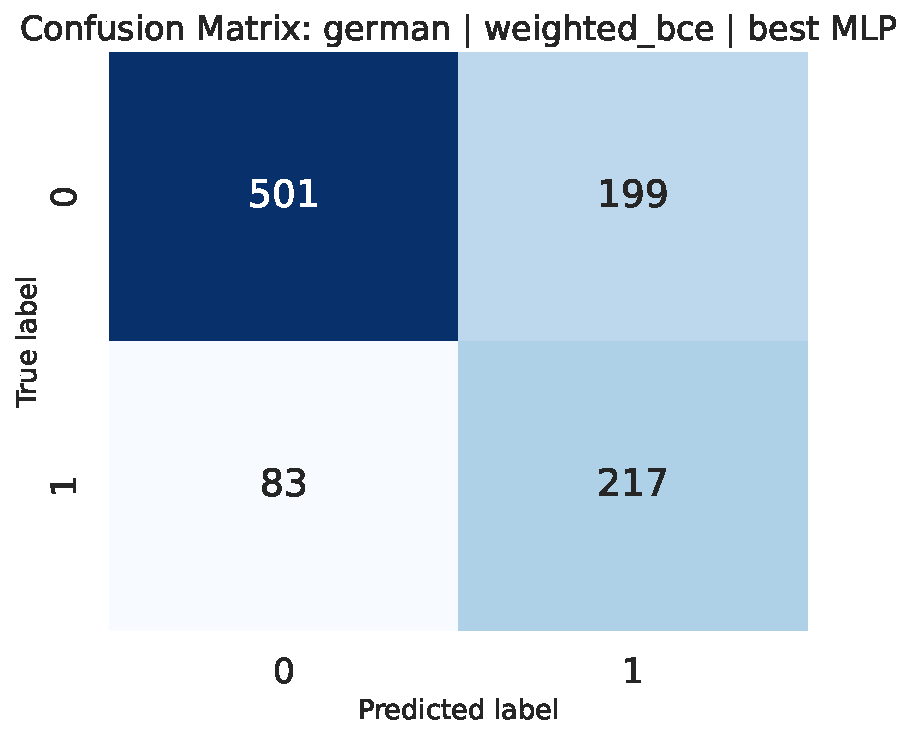
\includegraphics[width=\textwidth]{confusion_matrix_german_weighted_bce.pdf}
    \caption{German best model}
\end{subfigure}
\caption{Confusion matrices for the strongest aggregate configuration in each dataset.}
\label{fig:best-confusion}
\end{figure}

\subsection*{SHAP-Based Post-hoc Explainability}
The SHAP summary table highlights a compact, dataset-specific explanation pattern. For Australian MLP + focal loss, the strongest features were \texttt{A4}, \texttt{A7\_1}, \texttt{A7\_0}, and \texttt{A9}. For Default Credit GRU baseline, repayment-status variables dominated, especially \texttt{PAY\_0}. For German MLP + weighted BCE, \texttt{G0} was by far the strongest feature, followed by \texttt{G2} and \texttt{G1}. Table~\ref{tab:shap-summary} lists the top five features for each best configuration.

\begin{table}[htbp]
\centering
\small
\caption{Top five SHAP features for the best aggregate configuration in each dataset.}
\label{tab:shap-summary}
\begin{tabular}{lllrr}
\toprule
Dataset & Condition & Feature & Importance & Explainer \\
\midrule
australian & focal\_loss & A4 & 0.0433 & KernelExplainer \\
australian & focal\_loss & A7\_1 & 0.0393 & KernelExplainer \\
australian & focal\_loss & A7\_0 & 0.0347 & KernelExplainer \\
australian & focal\_loss & A9 & 0.0293 & KernelExplainer \\
australian & focal\_loss & A6 & 0.0152 & KernelExplainer \\
default\_credit & baseline & PAY\_0 & 0.0819 & KernelExplainer \\
default\_credit & baseline & LIMIT\_BAL & 0.0170 & KernelExplainer \\
default\_credit & baseline & MARRIAGE\_2 & 0.0133 & KernelExplainer \\
default\_credit & baseline & PAY\_4 & 0.0126 & KernelExplainer \\
default\_credit & baseline & PAY\_3 & 0.0117 & KernelExplainer \\
german & weighted\_bce & G0 & 0.1090 & KernelExplainer \\
german & weighted\_bce & G2 & 0.0448 & KernelExplainer \\
german & weighted\_bce & G1 & 0.0362 & KernelExplainer \\
german & weighted\_bce & G4 & 0.0305 & KernelExplainer \\
german & weighted\_bce & G15 & 0.0254 & KernelExplainer \\
\bottomrule
\end{tabular}
\end{table}

\subsection*{Selected Statistical Significance Results}
Because the full paired-test matrix is large, Table~\ref{tab:stats-summary} reports the most decision-relevant Wilcoxon comparisons. The pattern is consistent with the descriptive tables: SMOTE-ENN is frequently and significantly weaker than focal loss or weighted BCE on PR-AUC and balanced accuracy, especially for Default Credit and German MLP/LSTM settings.

\begin{table}[htbp]
\centering
\small
\caption{Representative statistically significant Wilcoxon results (\(p < 0.05\)).}
\label{tab:stats-summary}
\begin{tabular}{p{2.2cm}p{1.2cm}p{3.2cm}p{2.1cm}p{1.4cm}}
\toprule
Dataset & Model & Comparison & Metric & \(p\)-value \\
\midrule
Australian & GRU & smoteenn vs focal\_loss & PR-AUC & 0.0195 \\
Australian & LSTM & baseline vs smoteenn & PR-AUC & 0.0195 \\
Australian & MLP & smoteenn vs focal\_loss & balanced accuracy & 0.0195 \\
Default Credit & GRU & baseline vs smoteenn & PR-AUC & 0.0020 \\
Default Credit & LSTM & smoteenn vs weighted\_bce & PR-AUC & 0.0020 \\
Default Credit & MLP & smoteenn vs focal\_loss & PR-AUC & 0.0020 \\
German & LSTM & baseline vs weighted\_bce & PR-AUC & 0.0273 \\
German & MLP & baseline vs smoteenn & PR-AUC & 0.0195 \\
German & MLP & smoteenn vs weighted\_bce & PR-AUC & 0.0371 \\
\bottomrule
\end{tabular}
\end{table}

\section{Discussion}
The expanded experiment provides a clear answer to the research question. SMOTE-ENN did \emph{not} generalize as the strongest imbalance-handling strategy across datasets. Instead, the evidence supports a dataset-dependent story in which loss-based methods were more reliable overall. On Australian, focal loss produced the strongest aggregate model. On German, weighted BCE produced the best PR-AUC while focal loss produced the best balanced accuracy. On Default Credit, the baseline GRU remained best by PR-AUC, but both focal loss and weighted BCE improved balanced accuracy substantially without any help from SMOTE-ENN.

This pattern matters because it separates ranking quality from thresholded class balance. On heavily imbalanced data, a model can preserve high accuracy and specificity while still under-serving the minority class. That is exactly what happened in Default Credit baseline models. Weighted BCE and focal loss partially corrected that issue, whereas SMOTE-ENN often damaged PR-AUC instead. The most plausible explanation is the one already hinted at in the Assignment 2 reproduction: altering the training distribution through synthetic oversampling and ENN cleaning may simplify optimization while reducing fidelity to the original validation distribution.

The study also has important limitations, all of which are explicitly documented in the saved report summary. LSTM and GRU were applied to static tabular data through a feature-as-sequence representation rather than true temporal structure. The Australian and German datasets are relatively small, so fold-level variance remains meaningful. SHAP estimates depend on explainer compatibility and sample size. Finally, early stopping and runtime constraints affect the exact number of epochs seen by each model.

\section{Conclusion}
This Assignment 3 expansion does not support the claim that SMOTE-ENN is a robust improvement for deep-learning credit-risk prediction. Across three datasets and 36 model-condition combinations, loss-based methods matched or outperformed SMOTE-ENN on PR-AUC in all three datasets, while SMOTE-ENN was best in none. The strongest overall configurations were MLP + focal loss for Australian, GRU baseline for Default Credit, and MLP + weighted BCE for German.

The more defensible conclusion is therefore not that one imbalance method dominates universally, but that the best strategy depends on the dataset and the metric of interest. Still, the evidence in this study is more favorable to loss-level reweighting than to SMOTE-ENN, especially when the goal is to preserve generalization on the original class distribution while retaining interpretable post-hoc explanations through SHAP.

\section{References}
\begin{thebibliography}{9}

\bibitem{aruleba2025}
I. Aruleba and Y. Sun,
``Enhanced credit risk prediction using deep learning and SMOTE-ENN resampling,''
\emph{Machine Learning with Applications},
vol. 21, Art. no. 100692, 2025.

\bibitem{uci-german}
UCI Machine Learning Repository,
``Statlog (German Credit Data).''
\texttt{https://archive.ics.uci.edu/}

\bibitem{uci-australian}
UCI Machine Learning Repository,
``Statlog (Australian Credit Approval).''
\texttt{https://archive.ics.uci.edu/}

\bibitem{uci-default}
UCI Machine Learning Repository,
``Default of Credit Card Clients Dataset.''
\texttt{https://archive.ics.uci.edu/}

\bibitem{smoteenn-docs}
imbalanced-learn documentation,
``SMOTEENN.''
\texttt{https://imbalanced-learn.org/}

\bibitem{focal-loss}
T.-Y. Lin, P. Goyal, R. Girshick, K. He, and P. Dollar,
``Focal Loss for Dense Object Detection,''
in \emph{Proceedings of the IEEE International Conference on Computer Vision (ICCV)}, 2017.

\bibitem{shap}
S. M. Lundberg and S.-I. Lee,
``A Unified Approach to Interpreting Model Predictions,''
in \emph{Advances in Neural Information Processing Systems}, 2017.

\end{thebibliography}

\end{document}
